\section{Vue générale de la plate-forme}

Le projet {\it De Stijl} est une plate-forme de contrôle d'un robot mobile développée au département Génie \'Electronique et Informatique.  Les éléments constituant la plate-forme sont fournis et ont été testés de manière unitaire, mais nous ne garantissons pas un fonctionnement parfait. Toutes suggestions, corrections et modifications seront appréciées pour faire évoluer ce TP. Vous pouvez soumettre vos corrections (sujet, code ou autre) via le dépôt \href{https://github.com/INSA-GEI/dumber/}{GitHub}.

\subsection{\'Eléments de la plate-forme}

La plate-forme est constituée de quatre éléments (voir figure~\ref{fig:vue_gen}) : 
\begin{enumerate}
\item {\bf L'arène :} Boîte rectangulaire de couleur grise, elle est le terrain dans lequel le robot évolue.% Deux zones de couleur y sont tracées pour représenter des objectifs à atteindre. 
\item {\bf Le robot mobile :} Robot deux roues embarquant un microcontrôleur et un ensemble de composants matériels nécessaires à son déplacement. L'intelligence embarquée est volontairement limitée au contrôle de son déplacement (contrôle des moteurs) et à des fonctionnalités pour connaître son état.
\item {\bf Le superviseur :} Entité principale de la plate-forme, elle est dédiée au contrôle et à la supervision du robot. Elle est couplée à une Webcam fixée au-dessus du terrain afin d'en faire une acquisition visuelle et de localiser le robot.
\item {\bf Le moniteur :} Entité entièrement logicielle et distante, son rôle est d'offrir une interface de contrôle pour l'utilisateur.\\
 \end{enumerate}

La communication entre les équipements est hétérogène et assurée par différents supports :
\begin{enumerate}
\item La communication entre le robot et le superviseur est réalisée par une liaison sans fils point à point à l'aide de modules XBee. Cette communication est vue comme une liaison série.
\item La communication entre le superviseur et le moniteur est réalisée par un socket. La liaison physique est assurée par WiFi.
\end{enumerate}


\begin{figure}[htbp]
\begin{center}
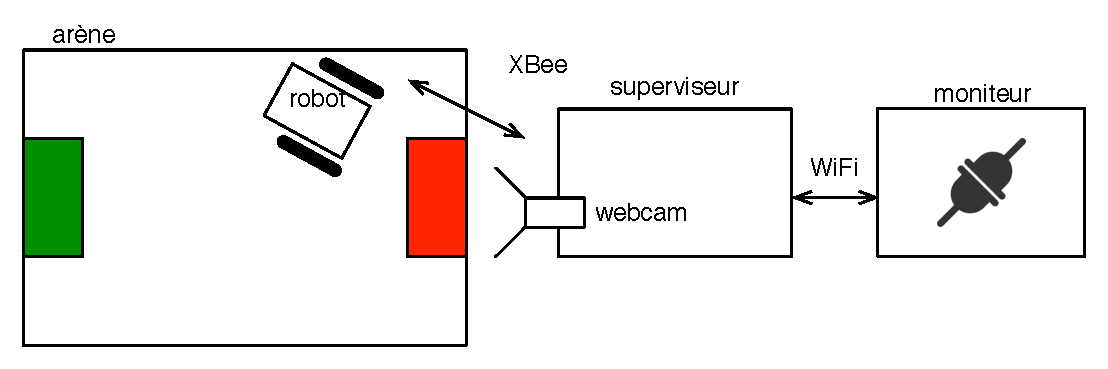
\includegraphics[scale=.6]{figures_pdf/schema_general2.pdf}
\caption{Vue générale de la plate-forme}
\label{fig:vue_gen}
\end{center}
\end{figure}
\FloatBarrier

 \subsubsection{Arène}

L'arène (voir figure~\ref{fig:arene}) a été réalisée dans les ateliers du département par J. Perez. C'est une boîte de 60$\times$80 cm en Medium et recouverte d'une peinture uniforme grise. Les bords sont peints en blanc. Deux zones distinctes sont peintes sur les bords opposés. L'une étant de couleur verte (ou orange) et l'autre de couleur rouge. Actuellement ces zones ne servent pas. %Ces zones sont désignées comme étant des buts.
 
 \begin{figure}[htbp]
\begin{center}
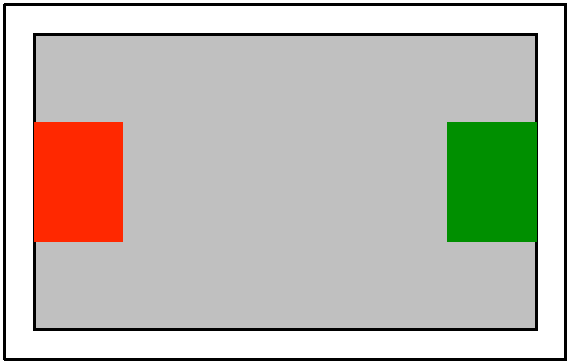
\includegraphics[scale=.6]{figures_pdf/arene.pdf}
\caption{Vue schématique de l'arène}
\label{fig:arene}
\end{center}
\end{figure}
\FloatBarrier

  \subsubsection{Robot}

La version 2.1 du robot a été conçue et réalisée par S. Di Mercurio. Schématiquement (figure~\ref{fig:robot}), le robot est constitué de deux moteurs, d'un microcontrôleur STM32F103RB et d'une puce Xbee assurant une liaison série point à point avec le superviseur. Chaque robot a un symbol différent sur le dos afin de l'identifier et de le localiser dans l'arène.

Le robot est mobile sur deux roues avec un patin. Le contrôle de la trajectoire est assuré par le contrôle en vitesse des moteurs. 

Le code embarqué dans les robots a été produit par S. Di Mercurio et L. Senaneuch. Il offre tous les services nécessaires pour contrôler le robot.
 
 \begin{figure}[htbp]
\begin{center}
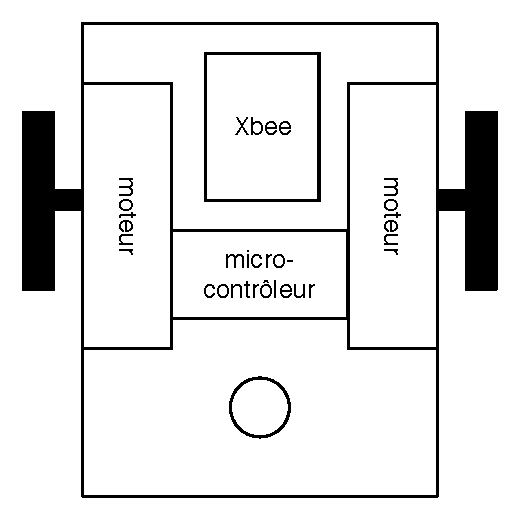
\includegraphics[scale=.6]{figures_pdf/schema_robot.pdf}
\caption{Vue schématique du robot}
\label{fig:robot}
\end{center}
\end{figure}
\FloatBarrier

\noindent\framebox[\textwidth]{
\begin{minipage}{0.9\textwidth}
{\bf Remarque :}  L'application que vous allez réaliser sera celle du superviseur. Vous ne toucherez pas au code embarqué dans le robot.
\end{minipage}
}\\

  \subsubsection{Superviseur}


Le superviseur orchestre le fonctionnement de la plate-forme en assurant le respect des contraintes temporelles du système. Il est déployé sur une Raspberry Pi 3B sur laquelle est installé un Ubuntu patché PREEMPT-RT avec l'extension mercury de Xenomai 3.0. Une Raspberry~Pi est un ordinateur à processeur ARM de taille réduite. La version 3B possède un processeur Broadcom BCM2837 64 bit à quatre cœurs ARM Cortex-A53 à 1,2 GHz, de puces WiFi 802.11n et Bluetooth 4.1. Un module Xbee a été ajouté pour communiquer avec le robot.

La webcam est intégrée au bloc du superviseur et est une caméra Raspberry.

\subsubsection{Moniteur}

Le moniteur permet à l'utilisateur de saisir les ordres que le robot doit réalisée et aussi de connaître l'état global du système. Il a été développé par S. Di~Mercurio en C\# à l'aide de \href{https://www.monodevelop.com}{MonoDevelop}. Le moniteur communique avec le superviseur via un socket. Le serveur est mis en place sur la superviseur et le moniteur en est le client.

\subsection{Bibliothèques logicielles}

\framebox[\textwidth]{
\begin{minipage}{0.9\textwidth}
Votre travail consistera à concevoir uniquement l'architecture logicielle du superviseur. Toutes les fonctions de traitement (communication, vidéo, etc.) {\bf ont déjà été implémentées} par L. Senaneuch et S. Di Mercurio. Vous n'aurez pas à modifier ce code, simplement à faire appel aux fonctions. Il n'en reste pas moins un gros travail d'architecte logiciel à faire.
\end{minipage}
}\\



Le code est disponible sur la branche stage du dépôt \href{https://github.com/INSA-GEI/dumber/}{GEI-INSA/dumber} sur GitHub . L'annexe~\ref{ann:diag_class} présente sous forme de diagramme de classes les bibliothèques disponibles.\\

Les fonctions de traitement sont réparties en cinq bibliothèques :
\begin{itemize}
	\item commonitor : services de communication entre le superviseur et le moniteur,
	\item comrobot : services de communication entre le superviseur et le robot,
	\item message : services définissant le format des messages entre le moniteur, le superviseur et le robot,
	\item camera : services de gestion de la caméra,
	\item img : services réalisant tous les traitements vidéos. \\
\end{itemize}

\framebox[\textwidth]{
\begin{minipage}{0.9\textwidth}
Toutes les bibliothèques ont été développées en C++, mais vous n'avez pas besoin de connaissances évoluées pour les utiliser (aucun support ne sera fourni par les encadrants pour le C++). Des explications sont fournies dans un document annexe pour manipuler les bibliothèques, mais d'une manière générale, vous n'avez pas besoin de connaissances évoluées en programmation objet pour les utiliser.
\end{minipage}
}
